\chapter{Semaphores} 
\label{chap:semaphores}

A semaphore is an important synchronisation tool.  The idea (and name) is
inspired by railway signalling, where a flag is raised to indicate that track
ahead can be entered, or lowered to indicate that the track ahead is occupied.
A train arriving at the section of track waits until the flag is up, enters
the section, and the flag is lowered again.  When the train leaves the section
of track, the flag is raised. 

A semaphore 
%% has a boolean variable, that indicates whether the flag is down.  It
has two operations:
%
\begin{description}
\item[\scalastyle{down()}:]
Wait until the flag is in the up position, and then put the flag down and
procced;

\item[\scalastyle{up()}:]
Put the flag up, to allow another thread to proceed.
\end{description}
%
The operations \SCALA{down} and \SCALA{up} are sometimes called \SCALA{P} and
\SCALA{V} (the initial letters of the Dutch words for the operations),
{\scalastyle wait} and \SCALA{signal}, or \SCALA{acquire} and
\SCALA{release}.

Figure~\ref{fig:semaphore-implementation} gives a straightforward
implementation of a semaphore using a JVM monitor.  The variable |isUp|
records whether the flag is currently in the up position.

%%%%%

\begin{figure}
\begin{scala}
/** A binary semaphore.
  * @param £isUp£ is the semaphore initially in the up state? */
class Semaphore(private var isUp: Boolean){
  def down() = synchronized{
    while(!isUp) wait()
    isUp = false
  }

  def up() = synchronized{
    require(!isUp); isUp = true; notify()
  }
}
\end{scala}
\caption{An implementation of a binary semaphore.}
\label{fig:semaphore-implementation}
\end{figure}

Note that the |up| operation requires that the semaphore is not already up.
This is a slightly non-standard design decisions: most implementations treat
the operation as a no-op in this case.  However, my experience is that trying
to put the semaphore up when it is already up is nearly always an error: a
signal gets lost.  I think it is better for the implementation to throw an
exception in this case, so that the error can be detected and removed.

\begin{instruction}
Make sure you understand how the implementation matches the informal
description given earlier.
\end{instruction}

In fact, many operating system kernels provide implementations of semaphores.
Those semaphores can then be used to implement other concurrency support, such
as monitors, within a programming language.

As with other concurrency mechanisms, semaphores can be used both for
providing mutual exclusion, which we will study in the next section, and for
waiting and signalling, which we will see subsequently.

%%%%%%%%%%%%%%%%%%%%%%%%%%%%%%%%%%%%%%%%%%%%%%%%%%%%%%%%%%%%

\section{Using a Semaphore for Mutual Exclusion}

One use of semaphores is to provide mutual exclusion.  

Such a semaphore is created with
\begin{scala}
  val mutex = new Semaphore(true)
\end{scala}
or
\begin{scala}
  val mutex = new MutexSemaphore
\end{scala}
%
using the definition
%
\begin{scala}
  class MutexSemaphore extends Semaphore(true)
\end{scala}
%
A thread entering the critical region executes
\begin{scala}
  mutex.down()
\end{scala}
%
This blocks if the semaphore is already down, i.e.~if another thread is in the
critical region.  In the initial state, the operation will not block. 
%
A thread leaving the critical region executes
\begin{scala}
  mutex.up()
\end{scala}
%
This unblocks a waiting thread (if there is one).

Figure~\ref{fig:semaphore-counter} gives an implementation of a counter that
uses a semaphore to provide mutual exclusion on the private variable~|x|.
Each operation initially performs a |down| on the semaphore, and performs an
|up| at the end.  Note that the |get| operation has to copy the value of~|x|
into a thread-local variable before raising the semaphore.

%%%%%

\begin{figure}
\begin{scala}
object Counter{
  private var x = 0
  
  private var mutex = new MutexSemaphore
    
  def inc() = { mutex.down(); x = x+1; mutex.up() }
  def dec() = { mutex.down(); x = x-1; mutex.up() }
  def get = { mutex.down(); val result = x; mutex.up(); result }
}
\end{scala}
\caption{An implementation of a counter using a semaphore for mutual
  exclusion.}
\label{fig:semaphore-counter}
\end{figure}

%%%%%

This technique can be used to provide mutual exclusion on arbitrary objects,
much like a |Lock|.

As with most concurrency primitives, it is possible to misuse semaphores.  For
exampe, consider the following code, where semaphore \SCALA{sem1} is used to
protect resource \SCALA{res1}, and semaphore \SCALA{sem2} is used to protect
resource \SCALA{res2}.
%
\begin{scala}
  val sem1 = MutexSemaphore(); val sem2 = MutexSemaphore()
  def t1 = thread{ sem1.down(); ...; sem2.down(); ... ; sem2.up(); ...; sem1.up() }
  def t2 = thread{ sem2.down(); ...; sem1.down(); ... ; sem1.up(); ...; sem2.up() }
  run(t1 || t2)
\end{scala}
%
This can deadlock.  Thread~|t1| can perform  |sem1.down()|, and thread~|t2| can
perform~|sem2.down()|.  Then, when each tries to perform |down| on the other
semaphore, they are blocked indefinitely. 

 % introduction; use for mutex
\section{Signalling Using Semaphores}

Recall, that a semaphore that is used to enforce mutual exclusion is initially
up.  A thread that enters the critical region does a \SCALA{down}, to block
other threads from entering.  When it leaves the critical region it does an
\SCALA{up}, to allow other threads to proceed.


By contrast a \emph{signalling semaphore} is initially down.  A thread can
send a signal by performing an \SCALA{up}.  A thread waits for a signal by
performing a \SCALA{down}.
\begin{scala}
  private val signal = new Semaphore(false)
  def signaller = thread{ ...; signal.up(); ... }
  def waiter = thread{ ...; signal.down(); ... }
\end{scala}  
Alternatively, the signalling semaphore can be created using
\begin{scala}
  private val signal = new SignallingSemaphore
\end{scala}
via the definition
\begin{scala}
  class SignallingSemaphore extends Semaphore(false)
\end{scala}
%
The \SCALA{waiter} cannot proceed before the signal is sent (but the
\SCALA{signaller} can proceed before the signal is received).
Note that the signal is received by only one other thread.  

%% Note also that if the |signaller| performs the signal before the |waiter|
%% is ready, the signal is not lost.

Semaphores and conditions are similar, in that each provides a signalling
mechanism.
%
The main difference is that a semaphore has a state: it is either up or down.
This means that if an |up| is performed before a thread is waiting, then the
signal is not lost.  
%
By contrast, if a signal is performed on a condition when
no thread is waiting, then the signal is lost: in such cases, it is often
appropriate to use the condition in combination with a boolean variable. 

Two threads can synchronise using a pair of signalling semaphores: each
signals to the other when it reaches the synchronisation point; neither
proceeds until it has received the signal from the other.
\begin{scala}
  val signal1 = new SignallingSemaphore; val signal2 = new SignallingSemaphore
  def t1 = thread{ ...; signal1.up(); signal2.down(); ... }
  def t2 = thread{ ...; signal2.up(); signal1.down(); ... }
\end{scala}


The above code works fine if the threads use the semaphores to synchronise
just once.  However, it can go wrong if the threads use the same semaphores to
synchronise multiple times.
%
\begin{scala}
  def t1 = thread{ for(i <- 1 to 2){ ...; signal1.up(); signal2.down(); ... } }
  def t2 = thread{ for(i <- 1 to 2){ ...; signal2.up(); signal1.down(); ... } }
\end{scala}
%
%% Consider an execution of the above where each thread should executes the loop
%% precisely twice.
The following sequence of events is possible, where the
subscripts represent the iteration number.
\[
\begin{align}
\sm{signal1.up}_1,\; \sm{signal2.up}_1,\; \sm{signal2.down}_1,\;
   \sm{signal1.up}_2.
\end{align}
\]
Thread~|t2| is suspended after performing its first signal, so that |t1|
performs its second signal \emph{before} |t2| consumes the first signal. 
With our implementation of semaphores, the precondition of |up| is not
satisfied, and an exception is thrown. 
If we had allowed an |up| when the semaphore is already up (and made it a
no-op), the execution would have continued something like:
\[
\begin{align}
%\sm{signal1.up}_1,\; \sm{signal2.up}_1,\; \sm{signal2.down}_1,\;
%   \sm{signal1.up}_2, \\
\ldots,\; \sm{signal1.down}_1,\; \sm{signal2.up}_2,\; \sm{signal2.down}_2.
\end{align}
\]
Here the second signal by |t1| is lost.  Subsequently, |t1| terminates, but
|t2| is stuck waiting for a second signal.

A solution is to reverse the order of events in one of the threads.
\begin{scala}
  def t1 = thread{ for(...){ ...; signal1.up(); signal2.down(); ... } }
  def t2 = thread{ for(...){ ...; signal1.down(); signal2.up(); ... } }
\end{scala}
%
We can reason as follows (recall the ``happens before'' relation $\prec$).
\[
\begin{array}{rcl@{\qquad}l}
\sm{signal1.up}_1 & \prec & \sm{signal1.down}_1 & 
  \mbox{(signal on {\scalashape signal1})} \\
 & \prec & \sm{signal2.up}_1 & \mbox{(program order for \SCALA{t2})} \\
 & \prec & \sm{signal2.down}_1 & \mbox{(signal on {\scalashape signal2})} \\
 & \prec & \sm{signal1.up}_2 & \mbox{(program order for \SCALA{t1})} \\
 & \prec & \ldots
\end{array}
\]
In particular, the events happen in the expected order, and neither thread
completes the synchronisation on the $n$th iteration before the other thread
has signalled on that iteration.
%
The precondition of |up| is satisfied since $\sm{signal1.down}_n \prec
\sm{signal1.up}_{n+1}$, for each~$n$, and similarly for |signal2|.

%%%%%%%%%%%%%%%%%%%%%%%%%%%%%%%%%%%%%%%%%%%%%%%%%%%%%%%%%%%%

\section{A Partial Queue Using Semaphores}

We will implement a partial queue using semaphores.  

If a |dequeue| finds that the queue is empty, it will wait for a signal on a
signalling semaphore |dequeueWait|.  When a subsequent |enqueue| signals on
this semaphore, it will indicate that the queue is now non-empty (in fact,
that the queue contains precisely one element), and the dequeue can proceed.

In addition, we have to protect the shared variables from  race conditions.  We
will use a |MutexSemaphore| for this. 

When an |enqueue| finishes, it will either (1)~signal on |dequeueWait| to a
waiting |dequeue| if there is one (and leave the mutex down), or (2)~lift the
mutex.  We record the number of waiting |dequeues| to support this.


%%%%%

\begin{slide}
\heading{Example: a partial queue using semaphores}

\begin{scala}
class SemaphorePartialQueue[T] extends PartialQueue[T]{
  /** The queue itself. */
  private val queue = new scala.collection.mutable.Queue[T]

  /** Number of waiting dequeues. */
  private var waitingDequeues = 0

  /** Semaphore to provide mutual exclusion. */
  private val mutex = new MutexSemaphore

  /** Semaphore on which a dequeue waits until the queue is non-empty. */
  private val dequeueWait = new SignallingSemaphore

  // Invariant: if waitingDequeues > 0 and mutex is up, then the queue is empty.
  ...
}
\end{scala}
\end{slide}

%%%%%

\begin{slide}
\heading{Example: a partial queue using semaphores}

\begin{scala}
  def enqueue(x: T) = {
    mutex.down
    queue.enqueue(x)
    if(waitingDequeues > 0) dequeueWait.up // pass the baton to a dequeue at (1)
    else mutex.up
  }

  def dequeue(): T = {
    mutex.down
    if(queue.isEmpty){  // have to wait
      waitingDequeues += 1; mutex.up
      dequeueWait.down                         // wait for signal (1)
      assert(queue.length == 1)
      waitingDequeues -= 1
    }
    val result = queue.dequeue(); mutex.up; result
  }
\end{scala}
\end{slide}

%%%%%

\begin{slide}
\heading{Passing the baton}

The technique used by |enqueue| is known as \emph{passing the baton}.  It
decides what sort of operation should run next ---either a waiting dequeue or
a new operation--- and ``passes it the baton'' by lifting the appropriate
semaphore. 

Note that when a thread passes the baton to a thread waiting on a signalling
semaphore, it leaves the mutex semaphore down: the latter takes over the
rights implied by possession of the mutex.  

By contrast, the waiting thread should lift the mutex before waiting,
otherwise the system will deadlock.

The technique of passing the baton is quite generally applicable.  Often the
current thread is in the best position to decide which thread can run next.
\end{slide}

%%%%%


\begin{slide}
\heading{Barrier synchronisation}

Recall that a barrier synchronisation can be used to synchronise $n>1$
threads.  Each thread in turn calls \SCALA{sync} on the barrier.  Once all
$n$ threads have called \SCALA{sync}, the threads can continue.
%% \end{slide}

%% %%%%%

%% \begin{slide}
%% \heading{Barrier synchronisation}

We define a class
\begin{scala}
class Barrier(n: Int){ def sync = { ... } }
\end{scala}%
%
to implement barrier synchronisation.  

We keep track of the number of threads currently waiting in a variable
\SCALA{waiting}.  We protect this using a mutex semaphore. 

We use a signalling semaphore \SCALA{waitSem} to block the first $n-1$
threads.  The $n$th thread signals on this semaphore to unblock
another thread, i.e.~passes it the baton.  That thread passes the
baton to another waiting thread (assuming $n \ge 3$), and so on.  The
final thread to be awoken raises the mutex, to pass the baton to a
thread on the next round.
\end{slide}


%%%%%

\begin{slide}
\heading{Barrier synchronisation}

\begin{scala}
class Barrier(n: Int){
  private var waiting = 0 // # threads waiting
  private val waitSem = new SignallingSemaphore
  private val mutex = new MutexSemaphore

  def sync = {
    mutex.down
    if(waiting == n-1) waitSem.up // start the waking up
    else{ 
      waiting += 1; mutex.up; waitSem.down  // wait until woken
      waiting -= 1
      if(waiting > 0) waitSem.up // pass baton to next waiting thread
      else mutex.up // pass baton to thread on next round.
    }
  }
}
\end{scala}

\end{slide}

%%%%%
\begin{slide}
\heading{Barrier synchronization}

\begin{itemize}
\item
The first $n-1$ threads  end up blocked on \SCALA{waitSem.down};

\item The $n$th thread performs \SCALA{waitSem.up}, to pass the baton to
another thread, and returns;

\item In turn, $n-2$ threads are woken, decrement \SCALA{waiting}, and wake up
the next thread;

\item The final thread to be woken, performs \SCALA{mutex.up} to allow the
following round of synchronisation to proceed.
\end{itemize}

Note that after the $n$th thread has called |sync|, no other thread can obtain
the mutex until the last thread exits, since \SCALA{mutex} remains down.
This prevents different rounds from interfering.
\end{slide}

%%%%%


%%%%%%%%%%%%%%%%%%%%%%%%%%%%%%%%%%%%%%%%%%%%%%%%%%%%%%%%%%%%

\begin{slide}
\heading{Example: a synchronous channel}

We will now implement a synchronous channel (suitable for use by multiple
senders and receivers) using semaphores.  We will need three signals for each
message, in the following order:
%
\begin{enumerate}
\item The sender will signal to the receiver that it has deposited a value, on
  semaphore |slotFull|.

\item The receiver will signal back to the sender on semaphore |continue|,
  thereby providing a synchronisation.

\item The sender will signal to the sender on the next round that the slot has
  been emptied, on semaphore |slotEmptied|.
\end{enumerate}
%
%These three semaphores will collectively provide mutual exclusion.
\end{slide}

%%%%%

\begin{slide}
\heading{Example: a synchronous channel}

\begin{center}
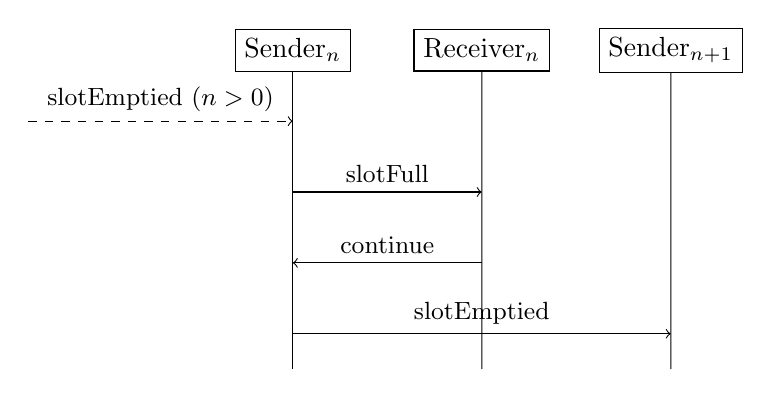
\begin{tikzpicture}[xscale = 1.2,yscale = 0.9]
\draw (0,0) node[draw](sender){ \scalacolour Sender$_n$ };
\draw (2,0) node[draw](receiver){ \scalacolour Receiver$_n$ };
\draw (4,0) node[draw](sender2){ \scalacolour Sender$_{n+1}$ };
\draw (sender) -- ++ (0,-4.5);
\draw (receiver) -- ++ (0,-4.5);
\draw (sender2) -- ++ (0,-4.5);
\draw[->,dashed] (-2.8,-1) -- 
  node[above] {\small\scalastyle slotEmptied ($n > 0$)} (0,-1);
\draw[->] (0,-2) -- node[above] { \small\scalastyle slotFull} (2,-2);
\draw[<-] (0,-3) -- node[above] { \small\scalastyle continue} (2,-3);
\draw[->] (0,-4) -- node[above] {\small\scalastyle slotEmptied} (4,-4);
\end{tikzpicture}
\end{center}
\end{slide}


%%%%%


\begin{slide}
\heading{Example: a synchronous channel}

\begin{scala}
class SyncChanSemaphores[A] extends SyncChanT[A]{  
  /** The current or previous value. */
  private var value = null.asInstanceOf[A]

  /** A semaphore for signalling to receiver that a value has been deposited. */
  private val slotFull = new SignallingSemaphore

  /** A semaphore for signalling to current sender that it can continue. */
  private val continue = new SignallingSemaphore

  /** A semaphore for signalling to the next sender that the previous value has
    * been read. */
  private val slotEmptied = new MutexSemaphore
  ...
}
\end{scala}
\end{slide}

%%%%%

\begin{slide}
\heading{Example: a synchronous channel}

The three semaphores will collectively provide mutual exclusion: when any
thread is active, all semaphores will be down; when no thread is active, a
single semaphore will be up.  Initially, just |slotEmptied| is up.

There is no need to have an extra |full| variable indicating that the current
value is valid: the |slotFull| and |slotEmptied| semaphores fulfil that role. 
\end{slide}

%%%%%

\begin{slide}
\heading{Example: a synchronous channel}

\begin{scala}
  def send(x: A) = {
    slotEmptied.down       // wait for previous value to be consumed (3)
    value = x               // deposit my value
    slotFull.up             // pass baton to receiver at (1)
    continue.down           // wait for receiver (2)
    slotEmptied.up          // pass baton to next sender at (3)
  }

  def receive: A = {
    slotFull.down           // wait for sender (1)
    val result = value      // take value
    continue.up             // pass baton to current sender at (2)
    result
  }
\end{scala}
\end{slide}

%%%%%

\begin{slide}
\heading{Example: a synchronous channel}

The signals must happen in the expected order:
\[
\begin{array}{rcl@{\qquad}l}
\sm{slotEmptied.down}_1 & \prec & \sm{slotFull.up}_1 & 
  \mbox{(program order for \SCALA{send})} \\
  & \prec & \sm{slotFull.down}_1 & \sm{(signal on {\scalashape slotFull})} \\
  & \prec & \sm{continue.up}_1 & \mbox{(program order for \SCALA{receive})} \\
  & \prec & \sm{continue.down}_1 & \sm{(signal on {\scalashape continue})} \\
  & \prec & \sm{slotEmptied.up}_1 & \mbox{(program order for \SCALA{send})} \\
  & \prec & \sm{slotEmptied.down}_2 & 
     \sm{(signal on {\scalashape slotEmptied})} \\
  & \prec & \ldots
\end{array}
\]

In particular, for each semaphore $s$,\, $s.\sm{down}_n \prec
s.\sm{up}_{n+1}$, so no signal is lost.
\end{slide}

%%%%%

\begin{slide}
\heading{Example: a synchronous channel}

Here's an incorrect version, where |receive| (rather than |send|) signals on
|slotEmptied|. 
%
\begin{scala}
  def send(x: A) = {
    slotEmptied.down       // wait for previous value to be consumed (3)
    value = x               // deposit my value
    slotFull.up             // pass baton to receiver (1)
    continue.down           // wait for receiver (2)
  }

  def receive: A = {
    slotFull.down           // wait for sender (1)
    val result = value      // take value
    continue.up             // pass baton to current sender (2)
    slotEmptied.up          // pass baton to next sender at (3)
    result
  }
\end{scala}
\end{slide}

%%%%%

\begin{slide}
\heading{Example: a synchronous channel}

With the version on the previous slide, suppose a |send| is suspended just
before performing |continue.down|.  Then the current receiver can signal on
|continue| and |slotEmptied|.  Then the following sender and receiver can run,
leading to a second |continue.up|, which breaks the precondition of |up|.  If
our implementation of semaphores had allowed such a second |up|, it would have
been a lost signal.
\end{slide}

%%%%%%%%%%%%%%%%%%%%%%%%%%%%%%%%%%%%%%%%%%%%%%%%%%%%%%%

\begin{slide}
\heading{Example: first-come-first-served mutual exclusion}

Consider a mechanism to allow clients to access a shared resource
under mutual exclusion.  Suppose we also want to ensure that clients
gain access in a first-come-first-served order.  (Note that this will have a
performance overhead, but might be desirable in some circumstances.)
%
We will implement this using semaphores. 

If a thread is forced to wait to access the resource, it will create a new
semaphore, place it in a queue, and then wait on it.  When a thread finishes
with the resource, it will pass the baton to the thread waiting on the first
semaphore in the queue (if there is one) by raising that semaphore.

We also need to record whether the resource is currently being used.  

And we need a semaphore to enforce mutual exclusion on the object's variables.
\end{slide}

%%%%%% 

\begin{slide}
\heading{Example: first-come-first-served mutual exclusion}

\begin{scala}
class MutexQueue{
  /** A queue of semaphores for waiting threads. */
  private val queue = new scala.collection.mutable.Queue[Semaphore]

  /** Is the resource busy? */
  private var busy = false

  /** Semaphore for mutual exclusion on this object's variables. */
  private val mutex = new MutexSemaphore

  // Invariant: if the mutex is up, and busy = false, then queue is empty.
  ...
}
\end{scala}
\end{slide}

%%%%%

\begin{slide}
\heading{Example: first-come-first-served mutual exclusion}

\begin{scala}
  def enter = {
    mutex.down
    if(busy){ // have to wait
      val sem = new SignallingSemaphore; queue.enqueue(sem)
      mutex.up; sem.down                  // wait turn (1)
    }
    else assert(queue.isEmpty)
    busy = true; mutex.up
  }

  def leave = {
    mutex.down; busy = false
    if(queue.nonEmpty){                 // wake up next thread at (1)
      val first = queue.dequeue(); first.up
    }
    else mutex.up
  }
\end{scala}
\end{slide}

%%%%%

\begin{slide}
\heading{Selective passing the baton}

This technique can be used in a number of scenarios to allow the current
thread to selectively pass the baton to a particular thread: each thread that
has to wait, creates a new semaphore, stores it, and waits on it.

Sometimes it is necessary to store some extra information with each such
semaphore, so that the current thread can choose between the waiting threads.
This choice should be made so that the thread that receives the signal can
then do something useful. 
\end{slide}
 % signalling; partial queue & passing the baton; barrier,
\section{A Synchronous Channel}

We  now implement a simple synchronous channel---similar to that in
earlier chapters---using semaphores.  We  need three signals for each
message, in the following order:
%
\begin{enumerate}
\item The sender  signals to the receiver that it has deposited a value, on
  semaphore |slotFull|.

\item The receiver  signals back to the sender on semaphore |continue|,
  thereby providing a synchronisation.

\item The sender signals to the sender on the next round that the slot has
  been emptied, on semaphore |slotEmptied|.
\end{enumerate}
%
%These three semaphores will collectively provide mutual exclusion.
Figure~\ref{fig:semaphore-syncChan-SD} illustrates the sequence of signals. 

%%%%%

\begin{figure}[hbtp]
\begin{center}
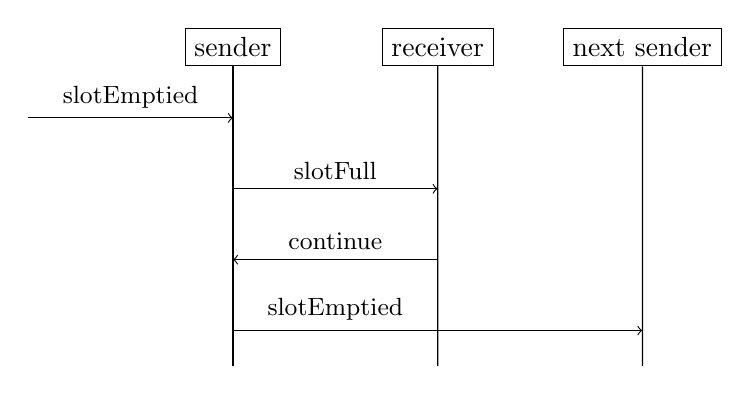
\begin{tikzpicture}[xscale = 1.3,yscale = 0.9]
\draw (0,0) node[draw](sender){sender};
\draw (2,0) node[draw](receiver){receiver};
\draw (4,0) node[draw](sender2){next sender};
\draw (sender) -- ++ (0,-4.5);
\draw (receiver) -- ++ (0,-4.5);
\draw (sender2) -- ++ (0,-4.5);
\draw[->] (-2.0,-1) -- 
  node[above] {\small\scalastyle slotEmptied} (0,-1);
\draw[->] (0,-2) -- node[above] { \small\scalastyle slotFull} (2,-2);
\draw[<-] (0,-3) -- node[above] { \small\scalastyle continue} (2,-3);
\draw[->] (0,-4) -- node[above, near start] {\small\scalastyle slotEmptied} (4,-4);
\end{tikzpicture}
\end{center}
\caption{Sequence diagram showing the sequence of signals in the
  semaphore-based implementation of a synchronous channel.}
\label{fig:semaphore-syncChan-SD} 
\end{figure}


%%%%%

\begin{figure}
\begin{scala}
class SemaphoreSyncChan[A] extends tacp.monitors.SyncChanT[A]{  
  /** The current or previous value. */
  private var value = null.asInstanceOf[A]

  /** A semaphore for signalling to receiver that a value has been deposited. */
  private val slotFull = new SignallingSemaphore

  /** A semaphore for signalling to current sender that it can continue. */
  private val continue = new SignallingSemaphore

  /** A semaphore for signalling to the next sender that the previous value has
    * been read. */
  private val slotEmptied = new MutexSemaphore

  /* Note: the semaphores together provide mutual exclusion. */

  def send(x: A) = {
    slotEmptied.down()      // Wait for previous value to be consumed (1).
    value = x               // Deposit my value.
    slotFull.up()           // Pass baton to receiver at (2).
    continue.down()         // Wait for receiver (3).
    slotEmptied.up()        // Pass baton to next sender at (1).
  }

  def receive(): A = {
    slotFull.down()         // Wait for sender (2).
    val result = value      // Take value.
    continue.up()           // Pass baton to current sender at (3).
    result
  }
}
\end{scala}
\caption{A synchronous channel implemented using semaphores.}
\label{fig:SemaphoreSyncChan}
\end{figure}

%%%%%

The implementation is in Figure~\ref{fig:SemaphoreSyncChan}.
The three semaphores collectively provide mutual exclusion: when any
thread is active, all semaphores are down; when no thread is active, a
single semaphore is up.  Initially, just |slotEmptied| is up.

Unlike the implementations in earlier chapters, there is no need to have an
extra |full| variable indicating that the current value is valid: the
|slotFull| and |slotEmptied| semaphores fulfil that role.


We can argue that the signals must happen in the expected order.  We write
``$\sm{slotEmptied.down}_1$'' for the first |down| performed on |slotEmptied|,
etc.  Then we can argue as follows, based on a combination of program order
for the two threads, and the fact that each |up| must precede the
corresponding |down| (except for the initial |down| on |slotEmptied|, since
that semaphore is initially in the \emph{up} state).  
\[
\begin{array}{rcl@{\qquad}l}
\sm{slotEmptied.down}_1 & \prec & \sm{slotFull.up}_1 & 
  \mbox{(program order for \SCALA{send})} \\
  & \prec & \sm{slotFull.down}_1 & \sm{(signal on {\scalashape slotFull})} \\
  & \prec & \sm{continue.up}_1 & \mbox{(program order for \SCALA{receive})} \\
  & \prec & \sm{continue.down}_1 & \sm{(signal on {\scalashape continue})} \\
  & \prec & \sm{slotEmptied.up}_1 & \mbox{(program order for \SCALA{send})} \\
  & \prec & \sm{slotEmptied.down}_2 & 
     \sm{(signal on {\scalashape slotEmptied})} \\
  & \prec & \ldots
\end{array}
\]
In particular, for each semaphore $s$,\, $s.\sm{down}_n \prec
s.\sm{up}_{n+1}$, for each~$n$, so the precondition of the |up| operation is
satisfied.

\begin{instruction}
Study the implementation, and make sure you understand why the semaphore
operations occur in the above order.
\end{instruction}

%%%%%

The signalling here is in a slightly different order from that in the
implementation using an SCL monitor in Section~\ref{sec:conditionsChan}.
There, the receiver---rather than the sender---signals to the next sender.
Figure~\ref{fig:SemaphoreSyncChan-incorrect} gives a corresponding signalling
strategy using semaphores---but it turns out that this is incorrect!

%%%%%

\begin{figure}
\begin{scala}
  def send(x: A) = {
    slotEmptied.down()       // Wait for previous value to be consumed (1).
    value = x               // Deposit my value.
    slotFull.up()             // Pass baton to receiver at (2).
    continue.down()           // Wait for receiver (3).
  }

  def receive(): A = {
    slotFull.down()           // Wait for sender (2).
    val result = value      // Take value.
    continue.up()             // Pass baton to current sender at (3).
    slotEmptied.up()          // Pass baton to next sender at (1).
    result
  }
\end{scala}
\caption{An incorrect implementation of a synchronous channel using
  semaphores.}
\label{fig:SemaphoreSyncChan-incorrect}
\end{figure}

%%%%%

With the version in Figure~\ref{fig:SemaphoreSyncChan-incorrect}, suppose a
|send| operation is suspended just before performing |continue.down()|.  Then
the current receiver can signal on |continue| and |slotEmptied|.  Then the
following sender and receiver can run, leading to a second |continue.up()|.
But thus breaks the precondition of |up|!  If our implementation of semaphores
had allowed such a second |up|, it would have been a lost signal.  The correct
implementation ensures a strict order in which critical events occur. 


%%%%%%%%%%%%%%%%%%%%%%%%%%%%%%%%%%%%%%%%%%%%%%%%%%%%%%%

\section{First-Come, First-Served Locking}
\label{sec:queueLock}

We now consider an implementation of a lock to allow threads to access a
shared resource under mutual exclusion.  However, we also want to ensure that
threads gain access in a first-come, first-served order (we will make clear
later precisely what we mean by this). 
% (Note that this will
% have a performance overhead, but might be desirable in some circumstances.)
%

Figure~\ref{fig:QueueLock} gives an implementation of such a lock, using
semaphores.  It uses a variable |busy| to record whether a thread currently
holds the lock.  If a thread is forced to wait to gain access to the resource,
it creates a new semaphore, places it in a queue, and then waits on it.  When
a thread finishes with the resource, it passes the baton to the thread waiting
on the first semaphore in the queue (if there is one) by raising that
semaphore.  The semaphore |mutex| enforces mutual exclusion on the object's
variables.

%%%%%

\begin{figure}
\begin{scala}
class QueueLock extends LockT{
  /** A queue of semaphores for waiting threads. */
  private val queue = new scala.collection.mutable.Queue[Semaphore]

  /** Is the resource busy? */
  private var busy = false

  /** Semaphore for mutual exclusion on this object's variables. */
  private val mutex = new MutexSemaphore

  /** Acquire the lock. */
  def acquire() = {
    mutex.down()
    if(busy || !queue.isEmpty){ // Thread has to wait.
      val sem = new SignallingSemaphore
      queue.enqueue(sem)
      mutex.up(); sem.down() // Wait for turn.
      assert(!busy)  
    }
    busy = true
    mutex.up()
  }

  /** Release the lock. */
  def release() = {
    mutex.down()
    busy = false
    if(queue.nonEmpty){ // Signal to next thread in £queue£.
      val first = queue.dequeue(); first.up()
    }
    else mutex.up()
  } 
}
\end{scala}
\caption{A lock providing first-come, first served access.}
\label{fig:QueueLock}
\end{figure}

%%%%%

\begin{instruction}
Study the details of the lock.
\end{instruction}

Threads that are forced to wait subsequently acquire the lock in the order in
which they add their semaphores to the queue.  This means that threads acquire
the lock in the order in which they acquire the |mutex| semaphore.  It is
reasonable to assume that threads use the resource protected by the lock for a
reasonable amount of time, normally longer than the time they spend running in
the |acquire| operation; thus the resource itself is the main bottleneck,
rather than the lock.  Thus if thread~$t_1$ calls |acquire| a reasonable time
before thread~$t_2$, we can expect $t_1$ to acquire the lock first.

We define the \emph{doorway period} to be the period during which a thread
registers its desire to acquire the lock, placing its semaphore in the queue
if necessary.  We can expect this period to be quite short.  By contrast, the
\emph{waiting period}, where a thread waits to receive a signal on its
semaphore, might be rather longer.  Our first-come, first-served property is
that if thread~$t_1$ completes its doorway period before~$t_2$, then $t_1$
will access the resource first.


This technique---where each thread creates a semaphore, stores it, and then
waits on it---can be used in a number of scenarios to allow the current
thread to selectively pass the baton to a particular thread.
%% : each thread that
%% has to wait, creates a new semaphore, stores it, and waits on it.
%
Sometimes it is necessary to store some extra information with each such
semaphore, so that the current thread can choose between the waiting threads.
This choice should be made so that the thread that receives the signal can
then do something useful. 

  % synchronous channel, queue-lock
% \input{semaphores-syncchan}
%\input{semaphores-readers-writers} -- cut, one example too many?


%%%%%%%%%%%%%%%%%%%%%%%%%%%%%%%%%%%%%%%%%%%%%%%%%%%%%%%


\section{Counting semaphores}

The semaphores we have seen so far have been binary: they have just two
states, up and down.

A counting semaphore has a non-negative integer as its state.
%
\begin{itemize}
\item
The \SCALA{down} operation waits until the value is strictly positive, and
decrements it;

\item
The \SCALA{up} operation increments the value, waking a process if necessary.
\end{itemize}
%
The value of the semaphore can be thought of as the number of \emph{permits}
available for |down| operations. 


%%%%%


\begin{scala}
class CountingSemaphore(private var permits: Int = 0){

  def down = synchronized{
    while(permits == 0) wait()
    permits -= 1
  }

  def up = synchronized{
    permits += 1
    notify()
  }
}
\end{scala}


%%%%%

We can implement a queue, using a counting semaphore to block attempts to
remove elements until the buffer is non-empty.

\begin{scala}
/** A queue implemented using a counting semaphore. */
class CountingSemaphorePartialQueue[T] extends PartialQueue[T]{
  /** The queue itself. */
  private val queue = new scala.collection.mutable.Queue[T]

  /** Semaphore for mutual exclusion on queue. */
  private val mutex = new MutexSemaphore

  /** Semaphore for dequeueing.  The state of the semaphore equals
    * queue.length. */
  private val size = new CountingSemaphore(0)
  ...
}
\end{scala}


\begin{scala}
  def enqueue(v: T) = {
    mutex.down
    queue.enqueue(v)
    size.up
    mutex.up
  }

  def dequeue(): T = {
    size.down
    mutex.down
    val result = queue.dequeue()
    mutex.up
    result
  }
\end{scala}


%%%%%

\heading{A partial queue}

Note that the order in which |dequeue| obtains the semaphores is
important.  If it were to obtain |mutex| first, and |queue| is empty,
then this would block |enqueue|, so the system would be deadlocked. 

\emph{Exercise:} adapt this example to produce a bounded buffer that cannot
hold more than $n$ pieces of data.

%%%%%%%%%%%%%%%%%%%%%%%%%%%%%%%%%%%%%%%%%%%%%%%%%%%%%%%


% \begin{scala}
% class Buff[T]{
%   private val queue = new scala.collection.mutable.Queue[T];
%   private val mutex = new Semaphore; 
%   private val size = new CountingSemaphore(0);
%   ...
% }
% \end{scala}
% %
% \SCALA{queue} holds the data.  

% \SCALA{mutex} is used to ensure mutual exclusion of operations upon
% \SCALA{queue}.  

% \SCALA{size} is a counting semaphore which stores the number of elements
% currently in \SCALA{queue}; it is used to block attempts to remove elements
% when its value is~$0$.
% \end{slide}

% %%%%%

% \begin{slide}
% \heading{An unbounded buffer}

% \begin{scala}
% class Buff[T]{
%   ...

%   def add(v:T) = {
%     mutex.down;
%     queue.enqueue(v);
%     size.up; mutex.up;
%   }

%   def remove:T = {
%     size.down; mutex down;
%     val result = queue.dequeue;
%     mutex.up; return result;
%   }
% }
% \end{scala}
% \end{slide}

%%%%%

% \begin{slide}
% \heading{A bounded buffer}

% \emph{Exercise:} adapt this example to produce a bounded buffer, that cannot
% hold more than $n$ pieces of data.
% \end{slide}

%%%%%%%%%%%%%%%%%%%%%%%%%%%%%%%%%%%%%%%%%%%%%%%%%%%%%%%%%%%%

\begin{slide}
\heading{Summary}

\begin{itemize}
\item
Semantics of semaphores;

\item
Implementing a semaphore using a monitor;

\item
Using a semaphore to enforce mutual exclusion;

\item
Dangers of deadlock;

\item
Using a semaphore for signalling;

\item
Examples;

\item
Passing the baton;

%% \item
%% Fairness;

\item
Counting semaphores.
\end{itemize}
\end{slide}


%%%%%%%%%%%%%%%%%%%%%%%%%%%%%%%%%%%%%%%%%%%%%%%%%%%%%%%

\exercises

Something using fine-grained locking.  Linked list?
